% =====================================================================
%  main.tex — Relazione progetto Secure Cloud Computing (UNISA)
% =====================================================================
\documentclass[12pt,a4paper,oneside]{report}

% ---------------------------------------------------------------------
%  Lingua, codifica, font
% ---------------------------------------------------------------------
\usepackage[utf8]{inputenc}
\usepackage[T1]{fontenc}
\usepackage[english]{babel}
\usepackage{lmodern}
\usepackage{microtype}

% ---------------------------------------------------------------------
%  Layout pagina e interlinea
% ---------------------------------------------------------------------
\usepackage[a4paper,top=2.2cm,bottom=2.2cm,left=2.2cm,right=2.2cm]{geometry}

\usepackage{setspace}
\setstretch{1.2}

\setlength{\parindent}{0pt}
\setlength{\parskip}{0.4em}

% ---------------------------------------------------------------------
%  Colori
% ---------------------------------------------------------------------
\usepackage[table]{xcolor}

% Blu ardesia, desaturato
\definecolor{accent}{HTML}{3D5A80}
% Grigio-azzurro appena percettibile per le righe alternate
\definecolor{softgrey}{HTML}{F3F5F8}

% ---------------------------------------------------------------------
%  Titoli e sezioni
% ---------------------------------------------------------------------
\usepackage{titlesec}

\titleformat{\chapter}[hang]
    {\normalfont\LARGE\bfseries\color{black}}
    {\thechapter}{15pt}{}

\titlespacing*{\chapter}{0pt}{-15pt}{25pt}

\titleformat{\section}
    {\normalfont\Large\bfseries\color{black}}
    {\thesection}{0.8em}{}

\titlespacing*{\section}{0pt}{2em}{0.8em}

\titleformat{\subsection}
    {\normalfont\large\bfseries}
    {\thesubsection}{0.8em}{}

\titlespacing*{\subsection}{0pt}{1.5em}{0.6em}

\setcounter{secnumdepth}{3}
\setcounter{tocdepth}{2}

% ---------------------------------------------------------------------
%  Intestazioni e piè di pagina
% ---------------------------------------------------------------------
\usepackage{fancyhdr}

\pagestyle{fancy}
\fancyhf{}

\fancyhead[L]{\small Secure Cloud Computing}
\fancyhead[R]{\small Cloud Architecture Document}

\fancyfoot[C]{\small\thepage}

\setlength{\headheight}{14pt}
\renewcommand{\headrulewidth}{0.3pt}
\renewcommand{\footrulewidth}{0pt}

\fancypagestyle{plain}{
    \fancyhf{}
    \fancyfoot[C]{\small\thepage}
    \renewcommand{\headrulewidth}{0pt}
}

% ---------------------------------------------------------------------
%  Tabelle
% ---------------------------------------------------------------------
\usepackage{array}
\usepackage{booktabs}
\usepackage{tabularx}

\renewcommand{\arraystretch}{1.35}
\setlength{\tabcolsep}{6pt}

% Elimina le strisce bianche tra le regole booktabs e le righe colorate
\setlength{\aboverulesep}{0pt}
\setlength{\belowrulesep}{0pt}

% Linee booktabs dello stesso colore dell'intestazione:
%  - \toprule si fonde con l'intestazione colorata
%  - \midrule invisibile (l'intestazione separa già)
%  - \bottomrule chiude la tabella con una linea sottile
\setlength{\heavyrulewidth}{0.8pt}
\setlength{\lightrulewidth}{0pt}
\setlength{\cmidrulewidth}{0.4pt}
\arrayrulecolor{accent}

% Colonne personalizzate per tabularx
\newcolumntype{Y}{>{\raggedright\arraybackslash}X}

% Intestazione delle tabelle
\newcommand{\tablehead}[1]{%
    \textcolor{white}{\bfseries #1}%
}

% ---------------------------------------------------------------------
%  Figure e didascalie
% ---------------------------------------------------------------------
\usepackage{graphicx}
\usepackage{float}
\usepackage{caption}

\captionsetup{
    font=small,
    labelfont=bf
}

% ---------------------------------------------------------------------
%  Liste
% ---------------------------------------------------------------------
\usepackage{enumitem}
\setlist{itemsep=2pt}

% ---------------------------------------------------------------------
%  Utility
% ---------------------------------------------------------------------
\usepackage[hidelinks]{hyperref}
\usepackage[english]{cleveref}
% =====================================================================
\begin{document}

% --- Parte iniziale (numerazione romana) ---
\pagenumbering{roman}

\hypersetup{pageanchor=false}
% =====================================================================
%  frontespizio.tex
% =====================================================================
\begin{titlepage}
\centering
\singlespacing

% --- Logo e ateneo ---------------------------------------------------

\includegraphics[width=0.28\linewidth]{attach/logo_standard.png}\par
\vspace{0.8cm}

{\LARGE\scshape Università degli Studi di Salerno\par}
\vspace{0.5cm}

{\large Department of Information and Electrical Engineering\\
and Applied Mathematics (DIEM)\par}
\vspace{0.3cm}
{\large Master's Degree in Computer Engineering\par}

\vfill

% --- Titolo ----------------------------------------------------------
{\color{accent}\rule{\linewidth}{0.8pt}}\par
\vspace{0.5cm}
{\Large\scshape Secure Cloud Computing\par}
\vspace{0.5cm}
{\fontsize{18}{24}\selectfont\bfseries
Cloud Architecture for Glucose Forecasting\\
in Type~1 Diabetes\par}
\vspace{0.4cm}
{\large\itshape Cloud Architecture Document\par}
\vspace{0.5cm}
{\color{accent}\rule{\linewidth}{0.8pt}}\par

\vfill

% --- Docente e studenti ----------------------------------------------
\begin{minipage}[t]{0.38\linewidth}
\raggedright
\textbf{Professor}\\[0.15cm]
Prof. Angelo Marcelli
\end{minipage}%
\hfill
\begin{minipage}[t]{0.58\linewidth}
\raggedleft
\textbf{Students}\\[0.15cm]
\begin{tabular}{@{}l@{\hspace{1.2em}}r@{}}
Giovanni Lamberti    & IE22700272\\
Luigi Montonetti     & IE22700055\\
Vittorio Postiglione & IE22700189
\end{tabular}
\end{minipage}

\vspace{1.5cm}

% --- Anno accademico -------------------------------------------------
{\large Academic Year 2026/2027\par}

\end{titlepage}
\hypersetup{pageanchor=true}
% =====================================================================
%  abstract.tex
% =====================================================================
\chapter*{Abstract}
\addcontentsline{toc}{chapter}{Abstract}
\thispagestyle{plain}

% Colonna di testo più stretta e centrata (rientro di 1.8 cm per lato)
\begin{list}{}{%
    \setlength{\leftmargin}{1.5cm}%
    \setlength{\rightmargin}{1.5cm}%
    \setlength{\itemsep}{0pt}%
    \setlength{\parsep}{0.8em}%
    \setlength{\topsep}{0pt}}
\item[]
{\color{accent}\rule{\linewidth}{0.8pt}}

\vspace{0.6em}

This document describes the cloud architecture of the software-as-a-service application for glucose forecasting in Type 1 diabetes, whose functional architecture was presented in the previous phase of the project. The functional components are mapped onto actual cloud computing mechanisms and architectures.

The system is divided into network zones, protected by two firewalls and separate logical network perimeters. A load balancer, together with an isolated identity zone, directs each user to the services assigned to their role. These services are stateless and can scale automatically. Data are stored in encrypted and replicated cloud storage devices, while model training takes place offline using a pseudonymized copy of the data.

The document also explains how the different mechanisms work together, describes the main system flows and discusses how the architecture meets the Service Level Agreement while protecting sensitive health data. The choice of specific technologies is left to the implementation phase.

\vspace{0.4em}
{\color{accent}\rule{\linewidth}{0.8pt}}

\vspace{0.2em}


\end{list}

% --- Corpo (numerazione araba) ---
\cleardoublepage
\tableofcontents
\cleardoublepage

\pagenumbering{arabic}

% =====================================================================
%  cloud_intro.tex
% =====================================================================
\chapter{Cloud architecture}
\label{ch:overview}

This document describes how the functional architecture can be deployed on a cloud
infrastructure. During this phase, the architecture is designed without referring
to any specific cloud provider or technology, as these choices will be made during
the implementation phase.

\Cref{fig:architecture} shows the logical structure of the cloud architecture.
The circles placed one on top of another represent services running in multiple
instances. The red arrows show the prediction path, which is the only flow that
must meet the one-second response time requirement.

\begin{figure}[H]
\centering
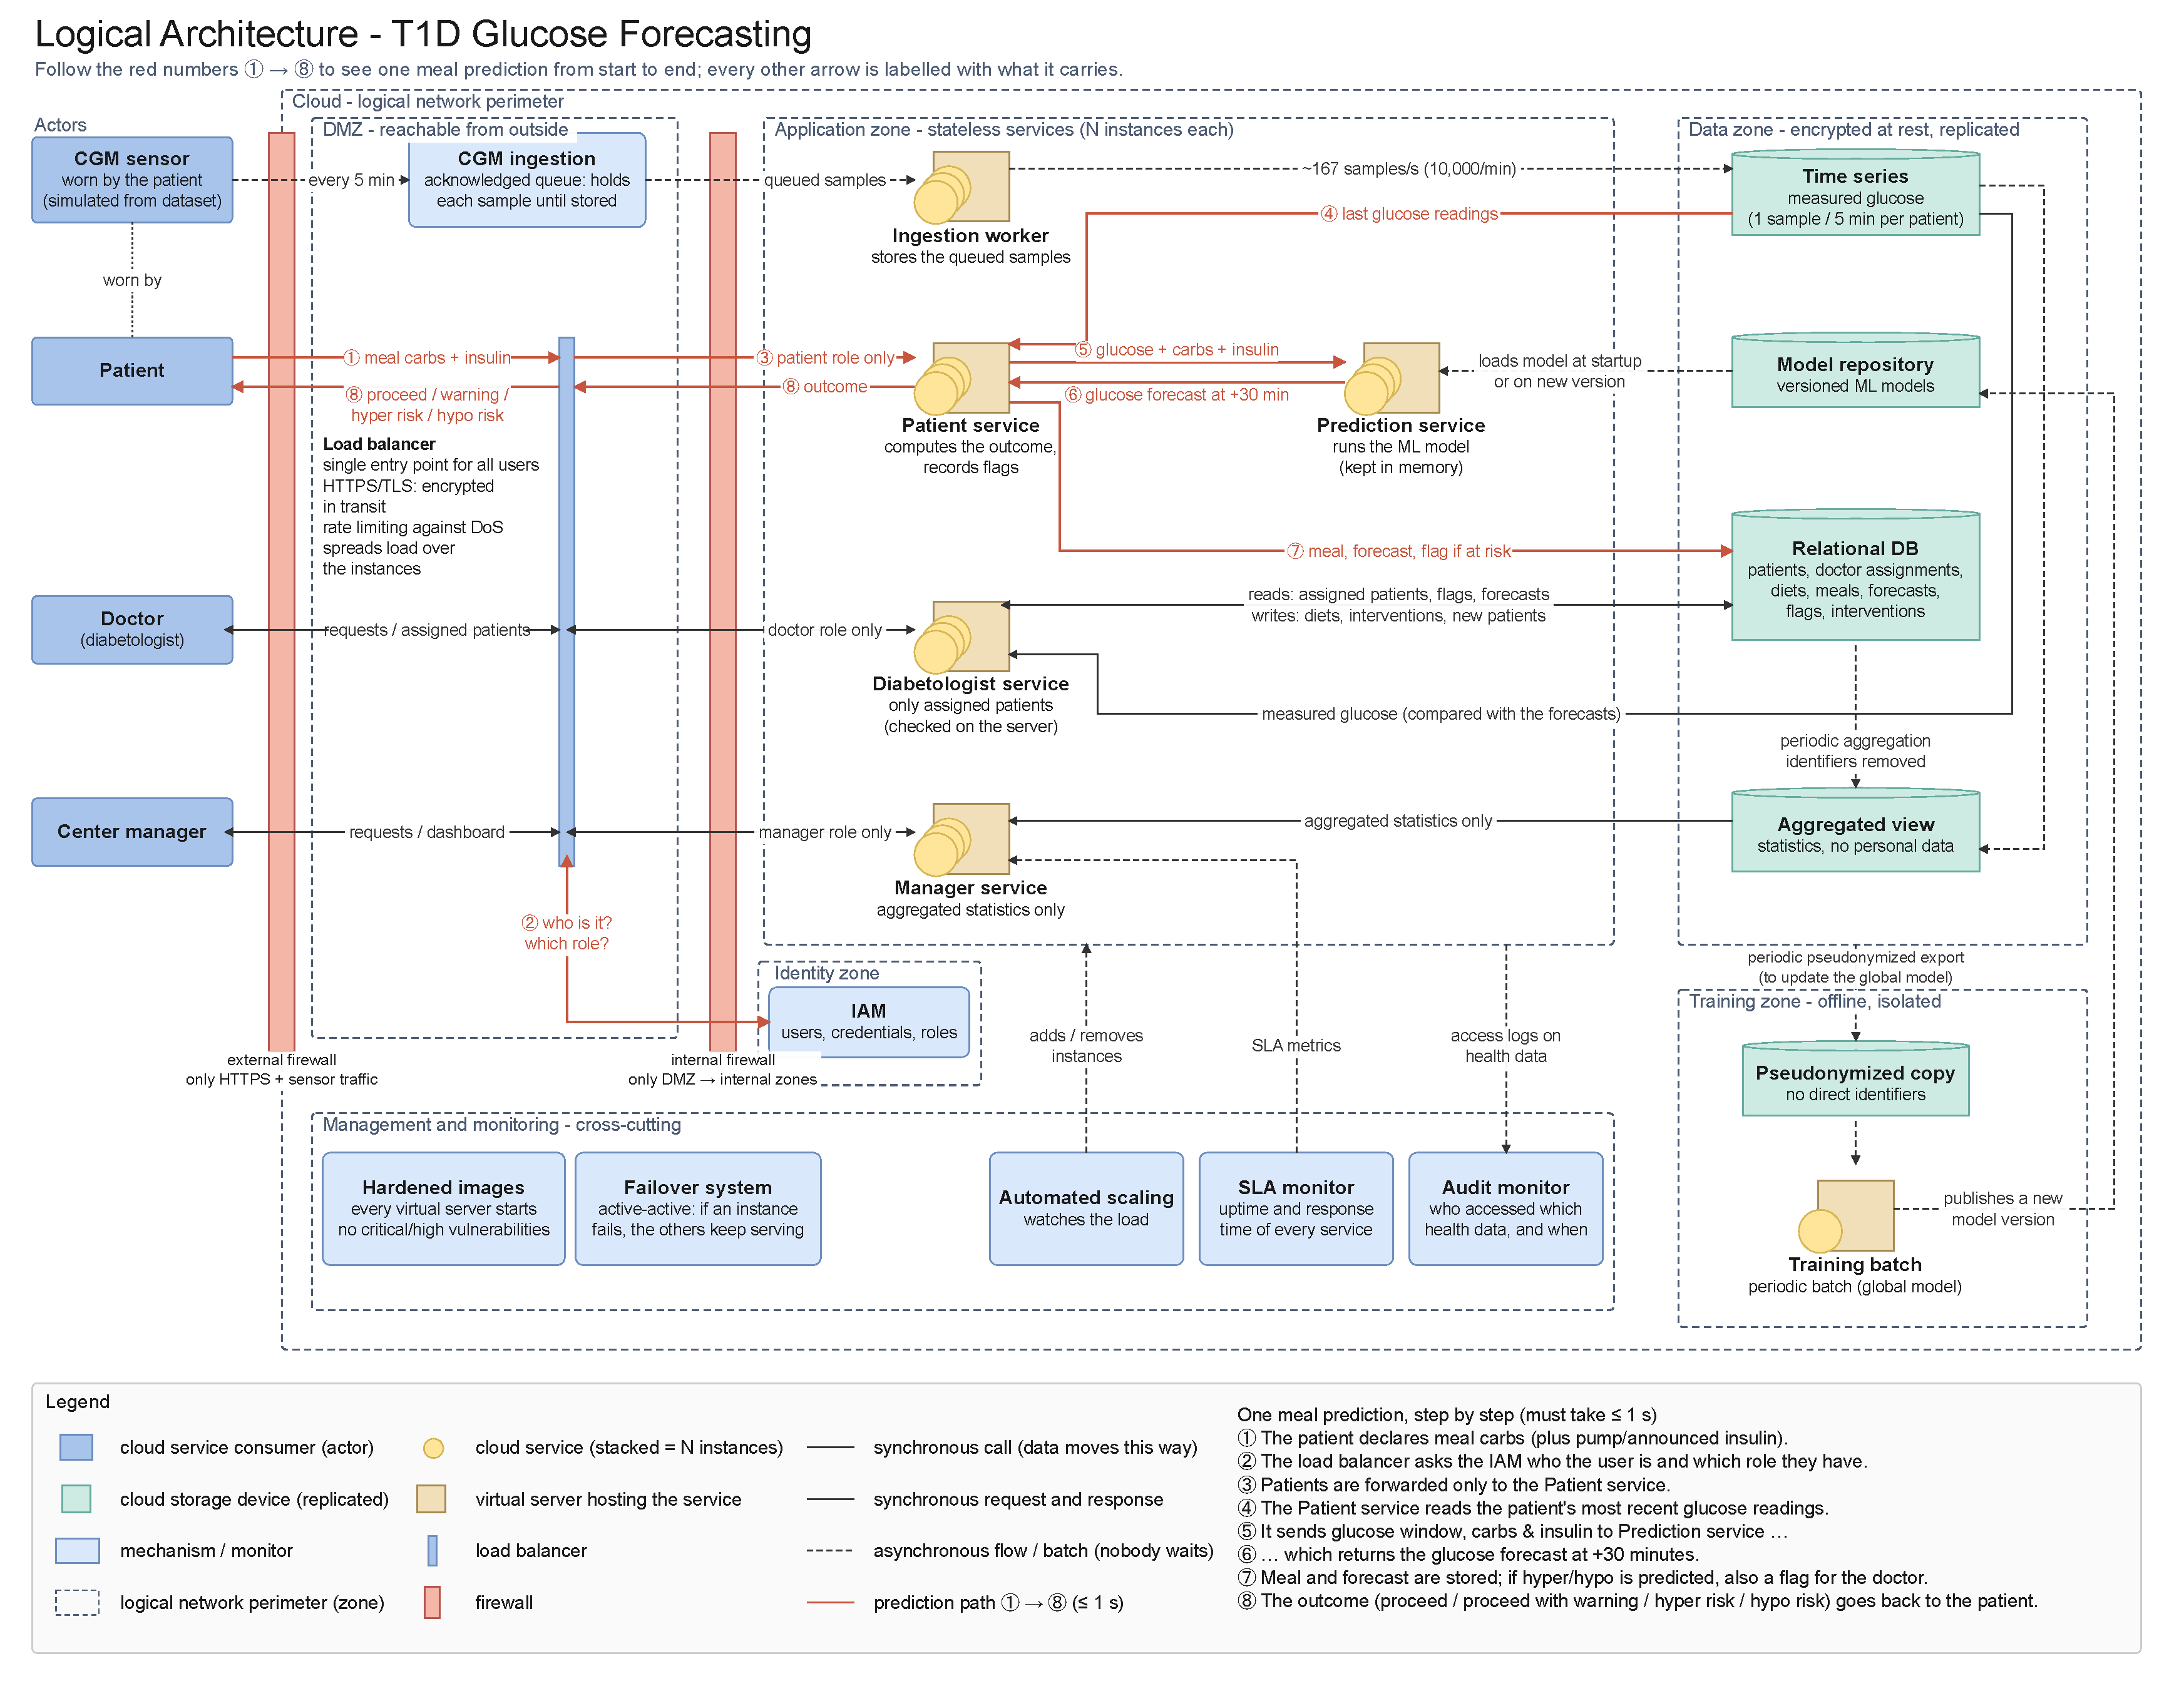
\includegraphics[width=\linewidth,height=0.92\textheight,keepaspectratio]{attach/arch.pdf}
\caption{Logical cloud architecture of the glucose forecasting service.}
\label{fig:architecture}
\end{figure}

The CGM sensor is represented as it would be in a real deployment: a separate
device worn by the patient that sends a new glucose sample every five minutes.
Since this project does not include a physical sensor, its behavior is simulated
by reading the samples from the dataset.

\section{Network zones}
\label{sec:zones}

The system is deployed within a logical network perimeter, which is further divided into separate zones, each one with its own perimeter (\cref{tab:zones}). 
Traffic is controlled by two
firewalls: the external firewall allows only HTTPS and sensor traffic to reach
the DMZ, while the internal firewall controls the traffic from the DMZ to the
internal zones, allowing only the connections required by the system.

\begin{table}[H]
\centering
\small
\rowcolors{2}{white}{softgrey}
\begin{tabularx}{\linewidth}{>{\raggedright\arraybackslash}p{3.4cm} Y >{\raggedright\arraybackslash}p{3.6cm}}
\toprule
\rowcolor{accent}
\tablehead{Zone} & \tablehead{Content} & \tablehead{Reachable from} \\
\midrule
DMZ                       & load balancer, CGM ingestion queue
                          & Internet, through the external firewall \\
Identity                  & IAM
                          & load balancer only \\
Application               & stateless services and ingestion worker
                          & DMZ, through the internal firewall \\
Data                      & encrypted and replicated storage devices
                          & application zone \\
Training                  & pseudonymized copy, training batch
                          & nobody (receives exports, publishes models) \\
Management and monitoring & hardened images, failover, scaling, SLA and
                            audit monitors
                          & administrators \\
\bottomrule
\end{tabularx}
\caption{Network zones of the architecture.}
\label{tab:zones}
\end{table}


The IAM is placed in a separate zone because it stores the credentials of all
users: even if an attacker manages to compromise a component in the
DMZ or the application zone, the IAM cannot be accessed directly from there.


The training zone is also kept isolated. This is because model training is an intensive task, has no strict timing requirements and does not require
access to the patients' identities.
% =====================================================================
%  cloud_mechanisms.tex
% =====================================================================
\chapter{Cloud mechanisms}
\label{ch:mechanisms}

\section{Infrastructure mechanisms}

\subsection{Logical network perimeter}

The logical network perimeter works at two levels. The outer perimeter
separates the system from the other consumers of the cloud, while the inner
perimeters divide it into the zones described in \cref{sec:zones}.
The data zone is protected by both firewalls and can only be reached from
the application zone. The training zone only receives the pseudonymized export
and publishes new models to the model repository.

\subsection{Virtual server}

Each service runs on its own virtual servers, created from hardened images.
In this way every service is sized independently and a fault in one service
does not affect the others.

\subsection{Cloud storage device}

The data are stored in different devices according to how they are used
and the level of security they require:

\begin{itemize}
    \item \textbf{time series}: stores the measured glucose values, one sample every five minutes per patient, about 167 writes per second;
    \item \textbf{relational database}: stores patient information, doctor assignments, diets,
          meals, forecasts, flags and interventions;
    \item \textbf{model repository}: stores the different model versions, so that every forecast
          can be traced to a model and a previous version can be restored;
    \item \textbf{aggregated view}: contains statistics without personal information and is the only storage reachable by the manager service;
    \item \textbf{pseudonymized copy}: is stored in the training zone and contains the data needed for training without direct identifiers.
\end{itemize}

\subsection{Resource replication}

Resource replication is used both for scaling and for recovery after a failure.
It creates new instances of virtual servers when needed and keeps a synchronized
copy of each storage device in the data zone.

\section{Specialized mechanisms}

\subsection{Load balancer}

The load balancer is the main entry point for all users. It handles HTTPS/TLS
connections, applies a rate limit to each client to help prevent denial-of-service
attacks and distributes requests across the available instances.

It also contacts the IAM to check the user's identity and role before forwarding
a request. Based on this information, the request is sent only to the service
assigned to that role (for example, a patient can never reach the diabetologist or the manager service).

\subsection{Automated scaling listener}


The scaling listener monitors the load of each service and adds or removes
instances when predefined thresholds are reached. The workload changes
throughout the day, with higher demand around breakfast, lunch and dinner.
To avoid wasting resources during quieter periods or having too few instances
during peak hours, the system can adjust the number of instances automatically.

At least two instances of each online service are always kept
available to support failover.

\subsection{Failover system}


The architecture uses an \textit{active-active} configuration, where all instances
handle requests at the same time. If one of them fails, the others continue
serving users while a replacement instance is started. 

We chose this approach
over active-passive because the instances are already needed to handle the
workload. There is also no need to wait for a standby instance to take over,
which helps keep outages short.

Storage devices also have a synchronized
replica ready to replace the primary one if it fails.

\subsection{SLA monitor}

The SLA monitor keeps track of the uptime and response time of each service.
It also sends an alert when a measured value gets close to its allowed limit.
The collected metrics are available to the manager service and displayed
in the center manager's dashboard.

\subsection{Audit monitor}

The audit monitor collects logs of all accesses to health data (who accessed which data, and
when) in a log that the services cannot modify, making it easier to identify
any improper access.

\section{Security mechanisms}
\label{sec:mech-security}

\subsection{Firewalls}


The external firewall allows only HTTPS traffic to reach the load balancer,
and sensor traffic to reach the CGM ingestion component. 

The internal firewall, instead,
controls the connections from the DMZ to the internal zones.

This prevents the
internal components from being directly exposed to the Internet.

\subsection{Encryption}

TLS protects the data in transit against eavesdropping and malicious
intermediaries. Data stored in the devices of the
data zone are also encrypted at rest. 

\subsection{Identity and access management}


The IAM stores user accounts, credentials and roles. It also handles the
identity checks requested by the load balancer. Passwords are always stored only as hashes. 

The load balancer checks the user's role,
while the diabetologist service performs an additional check to make sure
that the requested patient is actually assigned to that doctor.



\subsection{Hardened virtual server images}


Every virtual server starts from an image without unnecessary software,
services and accounts, and with no known critical or high vulnerabilities
(verified through automated vulnerability scanning). Instances created by
scaling or failover have the same protection level.


\subsection{Pseudonymization}

The data exported to the training zone have no direct identifiers. Since the training process does not need to know who the patients
are, this reduces the risk of exposing their identities if the training zone
is compromised.
% =====================================================================
%  cloud_flows.tex
% =====================================================================
\chapter{Main flows}
\label{ch:flows}

\section{Prediction path}
\label{sec:flow-prediction}

The main steps of the prediction process are shown in
\cref{fig:architecture}.

\begin{enumerate}
\item The patient enters the carbohydrate amount of the meal (supplemented by pump or announced insulin data).
\item The load balancer contacts the IAM to verify the user's identity
and role.
\item Based on the result, the patient is forwarded to the patient service.
\item The patient service retrieves the most recent glucose readings
from the time series.
\item It then sends the glucose window, together with the exogenous inputs
(carbohydrate intake and insulin), to the prediction service.
\item The prediction service returns the glucose forecast at thirty minutes.
\item The meal, exogenous inputs and forecast are stored in the relational
database. A flag is also added for the doctor if hyperglycemia or
hypoglycemia is predicted.
\item Finally, the outcome is sent back to the patient.
\end{enumerate}

To stay within one second, the model is loaded from the repository only when
an instance starts or when a new version is published, never during a request. 


\section{Ingestion of the glucose readings}
\label{sec:flow-ingestion}

In a real deployment, the sensors of about 50 000 patients generate around 10 000 samples per minute. The CGM ingestion component in the DMZ places each sample in a queue before storing it. The ingestion workers then take the samples from the queue and write them to the time series. If the storage slows down or a worker fails, the samples simply remain in the queue until they can be processed. This prevents data loss and keeps the ingestion process separate from the prediction path.

\section{Doctor access}

The doctor accesses the system through the diabetologist service and can only view the patients assigned to them. The service retrieves patient information, flags and forecasts from the relational database, as well as the measured glucose values from the time series. This gives the doctor the possibility to compare the forecasts with the actual readings. The doctor can also manage diets and interventions and register new patients. All accesses to health data are recorded by the audit monitor.

\section{Manager access}

The manager reaches only the manager service. It provides the aggregated view, which is periodically generated from operational data after removing personal identifiers. The manager can also view the metrics collected by the SLA monitor. This service has no access to personal data or to the operational databases.

\section{Training and publication of a new model}

The data zone periodically exports a pseudonymized copy of the data to the
training zone. The training batch runs periodically on this copy to update
the unified global model and publishes the new model version in the model
repository (newly registered patients do not require per-patient retraining).
The prediction instances load the new version one at a time, while the others
keep serving, so the service remains available during the update.
% =====================================================================
%  cloud_sla_security.tex
% =====================================================================
\chapter{Service Level Agreement and security}
\label{ch:sla}

\section{Cloud architectures}

The system combines different mechanisms to improve availability, scalability and fault tolerance:


\begin{itemize}
    \item \textbf{workload distribution} and \textbf{service load balancing}:
      each service runs in multiple instances, with requests distributed
      by a load balancer;
    \item \textbf{dynamic scalability}: horizontal scaling is performed by the
      automated scaling listener, and it is preferred to vertical scaling because it
      does not require a restart and improves redundancy;
    \item \textbf{redundant storage}: every storage device is paired with a secondary device that keeps a synchronized copy of the data;
    \item \textbf{zero downtime} and \textbf{dynamic failure detection and
      recovery}: when an instance fails, it is excluded from the service and automatically replaced by another one.
\end{itemize}


\section{How the architecture meets the SLA}

The uptime window ranges between 6:00 and 22:00. With sixteen hours of uptime per day, an availability of 99.5\% means that downtime must not exceed 4.8 minutes per day. In addition, a single outage must not last longer than 30 minutes, and on average the duration should remain within 3 minutes.

Because of these requirements, the time available to respond to failures is very limited and intervention should be managed automatically. \Cref{tab:sla-mapping} summarizes the
solutions adopted to meet the SLA requirements.


\begin{table}[H]
\centering
\small
\rowcolors{2}{white}{softgrey}
\begin{tabularx}{\linewidth}{>{\raggedright\arraybackslash}p{4cm} Y}
\toprule
\rowcolor{accent}
\tablehead{SLA parameter} & \tablehead{Mechanisms and architectures} \\
\midrule
Availability $\geq$ 99.5\%   & active-active failover, redundant storage,
                               at least two instances per service \\
Outage max 30 min, avg 3 min & automatic failure detection and recovery,
                               model updates one instance at a time  \\
Reliability $\geq$ 99.5\%    & stateless services (a failed request can be
                               repeated), queue that holds samples until stored \\
Response time $\leq$ 1 s     & model in memory, short prediction path,
                               dynamic horizontal scaling, SLA monitor \\
50\,000 customers, 5\,000 requests/min & load balancer, automated scaling listener,
                               ingestion separated from the requests \\
\bottomrule
\end{tabularx}
\caption{How the architecture meets the Service Level Agreement.}
\label{tab:sla-mapping}
\end{table}

The number of instances and the scaling thresholds will be fixed in the
implementation phase through \textit{stress testing}.

\section{Security}

The system manages health data, so security must be a main focus. In this section we consider the possible threats and show which mechanisms counter them.

\subsection{Threat agents}

The system is exposed to different possible threat agents:
\begin{itemize}
    \item an \textbf{anonymous attacker} without credentials, who tries to reach the service from the Internet;
    \item a \textbf{trusted attacker}, who is a legitimate user (such as a patient or a doctor) that tries to access unauthorized data;
    \item a \textbf{malicious insider}, such as an administrator who tries to read the health data;
    \item a \textbf{malicious service agent}, which is a program that intercepts or alters the traffic.
\end{itemize}

\subsection{Threats and countermeasures}

\begin{table}[H]
\centering
\small
\rowcolors{2}{white}{softgrey}
\begin{tabularx}{\linewidth}{>{\raggedright\arraybackslash}p{3.8cm} Y}
\toprule
\rowcolor{accent}
\tablehead{Threat} & \tablehead{Countermeasures} \\
\midrule
Traffic eavesdropping        & TLS on all the external and internal connections \\
Malicious intermediary       & TLS with server certificate\\
Denial of service            & external firewall, rate limiting, automated scaling,
                               queue for the sample readings \\
Insufficient authorization   & role-based routing on the load balancer, least privilege, check of the doctor-patient
                               assignment, aggregated view without personal data, audit monitor \\
Virtualization attack        & hardened images, one service per virtual server \\
Overlapping trust boundaries & separate perimeters, two firewalls, isolated identity zone \\
Malicious insider            & encryption at rest, pseudonymized training data, audit monitor, no direct access of administrators to the data \\
\bottomrule
\end{tabularx}
\caption{Security threats and countermeasures.}
\label{tab:threats}
\end{table}

The most relevant threats to this architecture are \textit{denial of service} and \textit{insufficient authorization}.

The first would leave the patient without support before a meal, so
the protection is provided at different levels through the firewall, load balancer and automatic scaling.

The second could expose sensitive health data. For this reason, the user's role is checked at the entry point, the diabetologist service verifies the patient's assignment, and all accesses are logged.
% =====================================================================
%  cloud_conclusions.tex
% =====================================================================
\chapter{Conclusions}
\label{ch:conclusions}

The architecture separates the system into zones protected by two firewalls,
isolates the identities and the training data, keeps the services stateless so
that they can be balanced and scaled, and treats the requests of the users and
the samples of the sensors on two different paths. Redundancy and automatic
recovery remove the single points of failure required by the SLA.

The next phase will choose the concrete technologies for each mechanism, fix
the scaling thresholds with a stress test, and scan the images for critical
and high vulnerabilities.


\end{document}